\section{问题三的建模与求解}
\label{sec:problem3}

问题三把问题二给出的广义标度律由描述工具转为决策工具：$N$、$D$、$Q$ 成为待定配置量，损失在算力约束下被最小化。约束一侧要写出三个资源要素各自的算力代价，结论一侧要回答结构性转移是否存在；后者的困难在于「结构」的数学化并不唯一，同一组最优解路径用不同判据去读会得到不同答案。以下依次给出优化模型与分段 KKT 解、锚点解与最优性核验、三种转移定义、成本函数与上下文长度的敏感性、与基线的对照以及配比的边际方向。全节数值一般保留四位小数，转移位置、隐含比值的漂移指数以及残差、预算违反量与乘子另给更多位数。

\subsection{优化模型与成本结构}
\label{subsec:q3-model}

在配比偏离取零（$\boldsymbol{z}_{\boldsymbol{p}}=\boldsymbol{0}$）的配置下，由式~\eqref{eq:q2-generalized} 得本问的优化问题
\begin{equation}
  \min_{N,D,Q}\ E+A\,N^{-\alpha}+B\,(D\,Q^{\gamma})^{-\beta}
  \qquad\text{s.t.}\qquad
  k\,N D+D\bigl[g(Q)-g(Q_0)\bigr]_{+}\le C,\quad Q_0\le Q\le 1,
  \label{eq:q3-problem}
\end{equation}
其中 $k=6+\eta L_{\text{ctx}}$，约束左端即三项算力开销：训练开销 $C_{\text{train}}=6ND$、注意力开销 $C_{\text{attn}}=\eta NDL_{\text{ctx}}$ 与质量提升开销 $C_{Q}=D[g(Q)-g(Q_0)]_{+}$，前两项合并为 $kND$。该族模型最初的用途是在参数量与数据量之间分配算力\citep{kaplan2020}，本问在其上增加了质量与上下文长度两个成本通道。

三项开销的缩放性质并不对称：$C_{\text{train}}$ 与 $C_{\text{attn}}$ 随 $N$、$D$ 同时缩放，$C_{Q}$ 只随 $D$ 缩放。由此 $C_{Q}/C_{\text{train}}=\Delta g/(6N)$ 只随 $N$ 反比，质量投入的预算份额随 $N^{*}$ 增大而被压缩；而 $C_{\text{attn}}/C_{\text{train}}=\eta L_{\text{ctx}}/6$ 与 $N$、$D$、$Q$ 无关，上下文长度的影响因此不落在两个规模变量之间的相对配比上。单位约定为：损失项以十亿为单位，成本项取绝对量纲（参数量与 token 数分别乘以 $10^{9}$，$\Delta g$ 亦然），故 $C_{\text{train}}=6N_BD_B\times10^{18}$ FLOPs；下文公式中的 $kN$、$N_{\text{abs}}$、$D_{\text{abs}}$ 均指绝对量纲。

配比 $\boldsymbol{p}$ 不作寻优变量。它经 $\exp(\boldsymbol{b}^{\top}\boldsymbol{z}_{\boldsymbol{p}})$ 线性进入有效 token 数，在单纯形约束下线性目标的最优解必落在顶点；建模阶段单独求解该角点问题，实测最大分量为 $0.9999999999999927$（全部分给 \texttt{dm\_mathematics}），已退化到数值精度以内。把配比联立只是重复该角点答案，且该答案对不可辨识的标度常数 $\kappa$ 敏感。本问据此固定配比，决策变量为 $(N,D,Q)$ 三个，KKT 驻点条件也是三个；领域边际方向在 \S\ref{subsec:q3-direction} 另报。

形状参数全部取自问题二的 B1 侧估计（表~\ref{tab:q2-params}）：$E=1.6898$、$A=0.3540$、$\alpha=0.3400$、$B=1.2403$、$\beta=0.2799$、$\gamma=0.9659$。B1 为 Pythia 的真实训练轨迹\citep{biderman2023pythia}。摘取时逐项核对，最大相对差小于 $10^{-15}$；截距另行复核，其 B1 侧与 B7 侧取值之差超过 $10^{-3}$，不存在误取。$\gamma$ 由附件 B7 的半合成网格反解，含 $\gamma$ 的读数带补充分析的性质。

题给的三类质量成本函数为指数型 $g=10^{7}\mathrm{e}^{6Q}$、幂函数型 $g=5\times10^{9}Q^{4}$ 与对数渐进型 $g=2\times10^{9}\ln(1+10Q)$。前两者的 $g'(Q)$ 无界递增，对数渐进型的 $g'=cr/(1+rQ)$ 单调递减并以 $c$ 为上界；这一差别既决定式~\eqref{eq:q3-R2} 下最优质量的取值，也是成本函数敏感性的来源。求解流程见图~\ref{fig:q3-framework}，三档锚点取 $C=10^{19}$、$10^{22}$、$10^{24}$ FLOPs。

\begin{figure}[htbp]
  \centering
  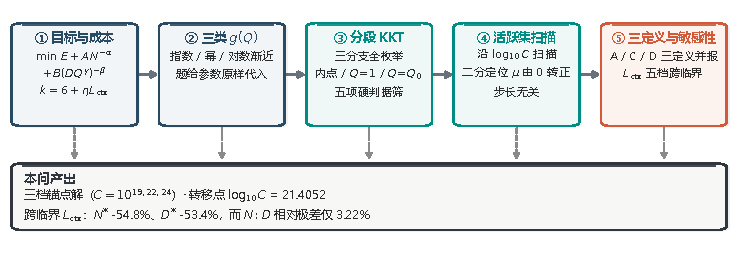
\includegraphics[width=0.96\linewidth]{figures/fig_framework_q3.pdf}
  \caption{问题三的建模与求解流程。上排五个环节依次为优化目标与成本结构、三类质量成本函数、
  三分支分段 KKT 求解、沿预算的活跃约束集扫描与转移定位、成本函数与上下文长度的敏感性；
  下方为本问产出，其中跨临界一行的两个百分数为 $L_{\text{ctx}}$ 由 2048 增至 131072 时的规模变化幅度。}
  \label{fig:q3-framework}
\end{figure}

\subsection{分段 KKT 约减与解析结构}
\label{subsec:q3-kkt}

内点一阶条件不能覆盖全部情形：预算充裕时，质量的内点最优会被推过上界 $Q=1$。实测比例比预期更极端，9 个「预算档 $\times$ 成本函数」组合中最优落于内点（$Q_0<Q^{*}<1$）的只有 2 个，即 $C=10^{19}$ 档的指数型（$0.6460$）与幂函数型（$0.5390$），其余 7 个位于上界 $Q^{*}=1$。故本问枚举三个分支：内点分支、上界分支（$Q=1$，$\Delta g$ 成为常数，未知量降为 $(N,D)$）与下界分支（$Q=Q_0$，$\Delta g=0$，即问题二的无质量投入配置）；每档取 KKT 判据全部通过且损失最小者。下界分支在三档中均未被选为最优，其在 $C=10^{19}$ 档的损失与后文诊断配置 M0o$'$ 逐位相同。

记 $S\equiv DQ^{\gamma}$。内点段由三个驻点条件消元得
\begin{equation}
  \alpha A\,N^{-\alpha}\bigl(k N+\Delta g\bigr)=\beta B\,S^{-\beta}\,k N,
  \label{eq:q3-R1}
\end{equation}
\begin{equation}
  \gamma\bigl(k N+\Delta g\bigr)=Q\,g'(Q).
  \label{eq:q3-R2}
\end{equation}
式~\eqref{eq:q3-R1} 由 $\partial N$ 与 $\partial D$ 消去预算乘子 $\lambda$ 得到，可读作单位成本上的边际损失下降在 $N$ 与 $D$ 之间相等。式~\eqref{eq:q3-R2} 由 $\partial D$ 与 $\partial Q$ 相除得到，相除时公共因子 $\beta B S^{-\beta}/D$ 被约去，$\lambda$ 与 $D$ 一并消失，故该式只含 $(N,Q)$，不含预算乘子与数据规模。由此得到两条独立核验路径。$\lambda$ 可由 $\partial N$ 单独解出，
\begin{equation}
  \lambda=\frac{\alpha A\,N^{-\alpha}}{k\,N_{\text{abs}}D_{\text{abs}}},
  \label{eq:q3-lambda}
\end{equation}
该式不含 $Q$ 与 $g'(Q)$，代回 $\partial D$ 即还原式~\eqref{eq:q3-R1}；实测三档 $\lambda$ 为 $2.4671\times10^{-20}$、$7.4101\times10^{-24}$ 与 $3.4636\times10^{-26}$，与由式~\eqref{eq:q3-R1} 独立解出的取值一致。残差方面，$C=10^{19}$ 档式~\eqref{eq:q3-R1} 与式~\eqref{eq:q3-R2} 的相对残差为 $9.29\times10^{-15}$ 与 $0.0$，后两档式~\eqref{eq:q3-R1} 为 $0.0$ 与 $2.11\times10^{-16}$；后两档落在边界分支上，式~\eqref{eq:q3-R2} 不再是条件（$Q$ 被钉在 1），其位置由 $dL/dQ\le0$ 与上界乘子非负的互补松弛取代，残差相应缺省。

式~\eqref{eq:q3-R2} 同时给出最优质量上升至饱和的机制：它是关于 $Q$ 的不动点条件，给定 $N$，仅当 $\gamma(kN+\Delta g(Q))$ 与 $Q\,g'(Q)$ 在 $(Q_0,1)$ 内有交点时内点解存在。$Q\,g'(Q)$ 在指数型与幂函数型下随 $Q$ 严格递增，右端随 $N$ 上升，故预算增加使交点右移、$Q^{*}$ 上升，直至交点越过上界而转入边界分支；对数渐进型的 $Q\,g'(Q)$ 以 $c$ 为上界，更早转入上界分支。边界段的乘子印证了分支归属：$C=10^{19}$ 档为 $3.44\times10^{-15}$，上界不活跃；高两档为 $0.0269$ 与 $0.0303$，上界活跃。三档的预算相对违反量为 $2.05\times10^{-16}$、$0.0$ 与 $1.34\times10^{-16}$，远低于预先设定的 $10^{-9}$ 容差。

\subsection{锚点解与最优性核验}
\label{subsec:q3-anchors}

上下文长度取附件 C7 的基准值 $2048$，成本函数取指数型，二者在 \S\ref{subsec:q3-sensitivity} 中另行扰动。三档解列于表~\ref{tab:q3-anchors}。

\begin{table}[htbp]
  \centering
  \caption{三档算力预算下的最优配置（$L_{\text{ctx}}=2048$，指数型成本函数；$N^{*}$、$D^{*}$ 以十亿计，
  预算违反量取相对形式 $(\text{cost}-C)/C$）}
  \label{tab:q3-anchors}
  \begin{tabular}{@{}lccc@{}}
    \toprule
    量 & $C=10^{19}$ & $C=10^{22}$ & $C=10^{24}$ \\
    \midrule
    分支            & 内点   & 上界   & 上界 \\
    活跃约束集       & 预算   & 预算、$Q\le1$ & 预算、$Q\le1$ \\
    $N^{*}$/B       & 0.2395 & 5.6475 & 40.7555 \\
    $D^{*}$/B       & 5.1662 & 249.0624 & 3771.0380 \\
    $Q^{*}$         & 0.6460 & 1.0000 & 1.0000 \\
    $D^{*}/N^{*}$   & 21.5727 & 44.1017 & 92.5284 \\
    损失            & 3.1468 & 2.1511 & 1.9139 \\
    $C_{\text{train}}$ 份额 & 0.7423 & 0.8439 & 0.9221 \\
    $C_{Q}$ 份额     & 0.2070 & 0.0984 & 0.0149 \\
    $C_{\text{attn}}$ 份额 & 0.0507 & 0.0576 & 0.0630 \\
    预算违反量       & $2.05\times10^{-16}$ & $0.0$ & $1.34\times10^{-16}$ \\
    \bottomrule
  \end{tabular}
\end{table}

表~\ref{tab:q3-anchors} 中有四项结构性读数。最优质量随预算上升并在 $C=10^{22}$ 档触到上界：$C=10^{19}$ 档 $Q^{*}=0.6460$ 为内点解，高两档为 $1.0000$；三档并非都落在上界，最低预算档的最优质量明确小于 1。质量投入的预算份额被单调压缩（$0.2070$、$0.0984$、$0.0149$），与 $C_{Q}/C_{\text{train}}=\Delta g/(6N)$ 的反比关系一致。$D^{*}/N^{*}$ 不是常数（$21.5727$、$44.1017$、$92.5284$），随预算单调上升。注意力开销的份额几乎不变（$0.0507$、$0.0576$、$0.0630$），其微弱上升全部来自 $C_{Q}$ 份额的下降。

外推性质需单独说明：$C=10^{22}$ 档的 $N^{*}$ 与 $D^{*}$ 为附件 B1 观测上界（$11.965825$B 与 $299.9$B）的 $0.4720$ 倍与 $0.8305$ 倍，仍在实测取值范围之内；$C=10^{24}$ 档为 $3.4060$ 倍与 $12.5743$ 倍，落在观测范围之外，该档读数应读作相同参数下的外推，不构成可靠预测。

最优性以预先设定的五项判据判定：预算相对违反量不超过 $10^{-9}$、驻点相对残差小于 $10^{-8}$、互补松弛、乘子非负、变量界。五项在三档锚点上全部通过；另沿 $\log_{10}C$ 由 $18.0$ 到 $25.0$ 以 $0.125$ 为步长取 57 个点扫描，分支枚举与 KKT 判据全部通过。表~\ref{tab:q3-kkt} 另列三条相互独立的核验与一次重复性检查。

\begin{table}[htbp]
  \centering
  \caption{最优性的独立核验（$\partial L/\partial N$、$\partial L/\partial D$、$\partial L/\partial Q$ 为对拉格朗日函数
  的中心差分重建结果，差分进化在整个可行域上独立求解同一目标）}
  \label{tab:q3-kkt}
  \small
  \begin{tabular}{@{}p{0.13\linewidth}p{0.37\linewidth}p{0.41\linewidth}@{}}
    \toprule
    核验路径 & 做法 & 实测结果 \\
    \midrule
    中心差分重建 & 直接对拉格朗日函数做数值微分，独立重建两个驻点等式，
      覆盖 9 个「预算档 $\times$ 成本函数」组合 &
      $\partial L/\partial N$ 与 $\partial L/\partial D$ 的相对残差均小于 $3.3\times10^{-8}$；
      内点段 $\partial L/\partial Q=0$，边界段 $\partial L/\partial Q\le0$ \\
    邻域采样 & 三档锚点邻域各取 4000 个可行点 & 更优者 0 例 \\
    全局数值对照 & 差分进化独立求解式~\eqref{eq:q3-problem}，与分支枚举解对照 &
      损失的相对差 $-1.35\times10^{-14}$、$-2.85\times10^{-14}$、$-6.53\times10^{-14}$ \\
    重复性 & 同一随机种子下重跑整轮求解 & 两次运行的输出逐位相同 \\
    \bottomrule
  \end{tabular}
\end{table}

三条核验落在不同环节：中心差分重建不经过分支枚举的代数约减，其边界段的 $\partial L/\partial Q\le0$ 正是上界乘子非负的等价陈述；邻域采样检验局部最优性；差分进化不依赖驻点条件，其与分支枚举解的损失相对差低于 $10^{-13}$，若枚举不完备，数值解应更优并出现可分辨的落差，实测没有出现。三档锚点解因此可视为式~\eqref{eq:q3-problem} 在给定参数下的最优解，其沿预算的完整路径见图~\ref{fig:q3-optimal-path}。

\begin{figure}[htbp]
  \centering
  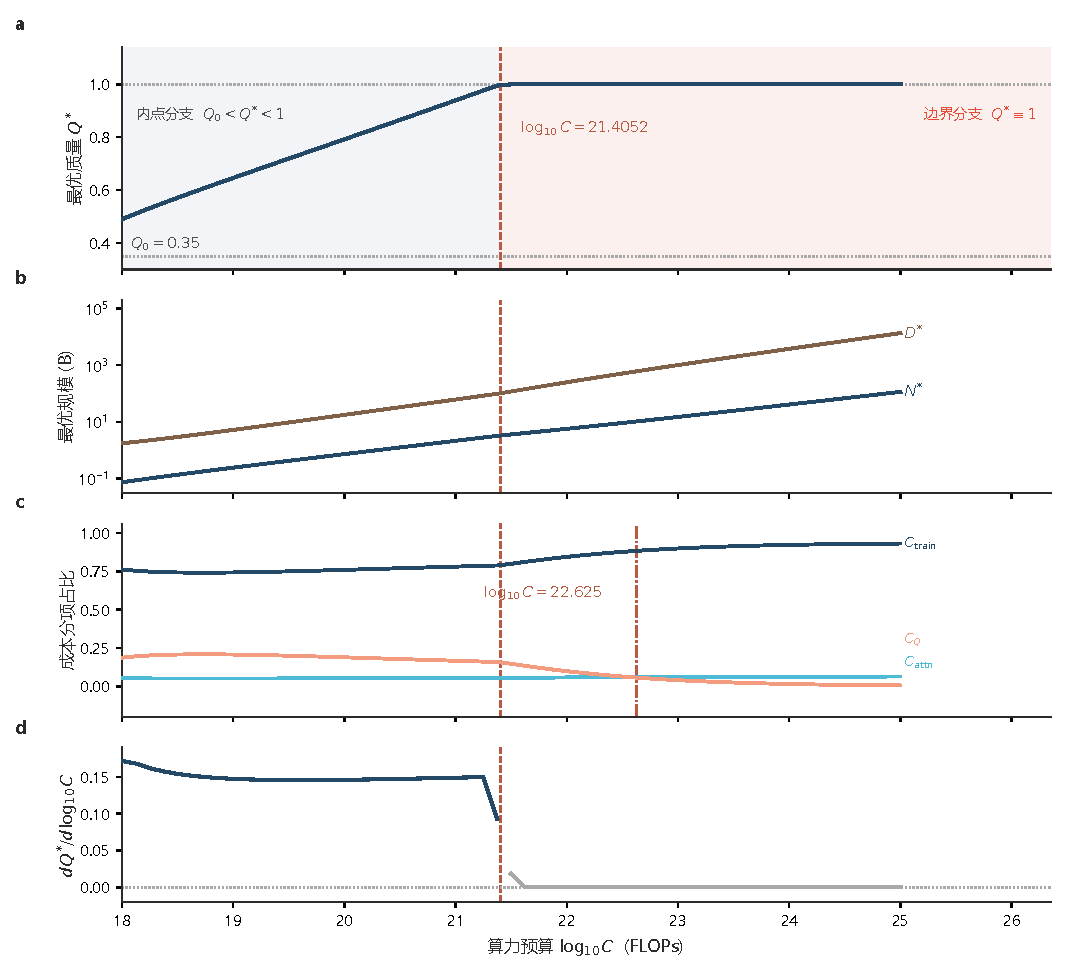
\includegraphics[width=0.86\linewidth]{figures/fig_q3_optimal_path.pdf}
  \caption{最优配置沿算力预算的路径，四联图共用横轴 $\log_{10}C$（FLOPs，18--25）。
  (a) 最优质量 $Q^{*}$，虚线为 $Q=1$ 与 $Q_0=0.35$，红色竖线为活跃约束集变化的位置 $\log_{10}C=21.4052$，
  左右两侧分别为内点分支与上界分支；(b) 最优规模 $N^{*}$ 与 $D^{*}$（B），纵轴为对数刻度；
  (c) 三项成本占预算的比例，点划线为 $C_{Q}$ 与 $C_{\text{attn}}$ 在 $\log_{10}C=22.625$ 处的排序翻转；
  (d) 饱和点附近的导数 $dQ^{*}/d\log_{10}C$，饱和前约为 $0.15$，饱和后为零，
  跨越饱和点的区段以灰线单列。}
  \label{fig:q3-optimal-path}
\end{figure}

\subsection{结构性转移的三种定义与识别}
\label{subsec:q3-transfer}

题目要求给出结构性转移的数学定义与识别方法。「结构」的数学化并不唯一，不同的数学化会给出不同的位置，甚至给出相反的存在性判断。

定义 A 把转移定义为最优解处活跃约束集 $\mathcal{A}(C)$ 的变化。本问中可变的约束元素只有质量的上界 $Q\le1$，该定义因而等价于问「质量投入是否由内部最优变为顶到上界」。识别方法是沿 $\log_{10}C$ 扫描活跃集与互补松弛乘子 $\mu$，转移点取 $\mu$ 由零转正处，实测位置为 $\log_{10}C=21.405181884765625$（区间 $[21.375,21.5]$，二分定位到 $10^{-4}$），活跃集由「预算」变为「预算、$Q\le1$」。该定义不引入阈值与数值微分，也不依赖扫描步长。

定义 C 把转移定义为成本分项占比的排序变化，实测排序由 $C_{\text{train}}|C_{Q}|C_{\text{attn}}$ 翻转为 $C_{\text{train}}|C_{\text{attn}}|C_{Q}$，位置为 $\log_{10}C=22.625$（由 $0.125$ 的网格读出），该点三个份额为 $0.8830$、$0.0567$ 与 $0.0603$；该定义不依赖阈值，但位置由步长给出。

定义 D 把转移定义为最优配置的突变，判据为相邻扫描点之间的 $|\Delta Q^{*}|$ 超过 $\delta=0.05$。实测结论随步长翻转：步长 $0.5$ 时最大 $|\Delta Q^{*}|$ 为 $0.0814$、有 7 个点越阈，判为存在；步长 $0.25$ 与 $0.125$ 时为 $0.0420$ 与 $0.0215$，判为不存在。成因是饱和前 $Q^{*}$ 光滑上升、斜率稳定在约 $+0.149$，一阶差分约等于斜率与步长之积，与固定阈值比较不是网格不变量。（另一种定义是最优解路径的不可微点，与定义 A 刻画同一事件但需数值微分，故不单列。）

三种定义的结果列于表~\ref{tab:q3-transfer}，对比见图~\ref{fig:q3-transition}。

\begin{table}[htbp]
  \centering
  \caption{结构性转移的三种定义与识别结果（$\delta$ 为定义 D 的份额突变阈值）}
  \label{tab:q3-transfer}
  \small
  \begin{tabular}{@{}p{0.20\linewidth}p{0.19\linewidth}cccl@{}}
    \toprule
    定义 & 判据 & 位置 $\log_{10}C$ & 依赖阈值 & 依赖步长 & 结论 \\
    \midrule
    A 活跃约束集变化（主） & 上界乘子 $\mu$ 由零转正 & 21.405181884765625 & 否 & 否 & 转移存在 \\
    C 成本分项占比排序变化 & 成本分项排序翻转 & 22.625 & 否 & 是 & 转移存在 \\
    D 分配份额突变（步长 0.125） & 相邻点 $|\Delta Q^{*}|>\delta$ & --- & 是 & 是 & 无转移 \\
    D 分配份额突变（步长 0.5） & 相邻点 $|\Delta Q^{*}|>\delta$ & --- & 是 & 是 & 转移存在 \\
    \bottomrule
  \end{tabular}
\end{table}

定义 A 问约束集是否改变，答曰发生且位置明确；定义 C 问成本结构是否重排，答曰发生，但位置晚于 A 约 1.2 个数量级；定义 D 问是否有突跳，细网格下答曰没有。三者并不冲突，因为所问的对象不同。主定义取 A：它在三种定义中唯一不需要自由参数，且直接对应「质量投入由内部最优变为顶到上界」这一策略层面的变化。定义 D 的翻转另给出一条方法论结论——把转移定义在一阶差分与固定阈值的比较上，结论会成为扫描步长的函数，不宜作为主定义。

合读的结论是转移存在，形态为连续饱和而非突跳。三条读数支持这一形态：饱和前 $dQ^{*}/d\log_{10}C$ 由 $0.1483$ 升至 $0.1500$（对应 $\log_{10}C$ 由 $20.875$ 至 $21.375$），饱和点之后恒为零，即在饱和处导数由正转零；跨越饱和点的 $\log_{10}C\in(21.375,21.5]$ 区段差商为 $0.0363$，既不是左导数也不是右导数，不参与符号判定，该区段单列排除后导数序列自 $21.625$ 起严格为零；定义 D 在细网格上判不出突变，与光滑饱和一致。

\begin{figure}[htbp]
  \centering
  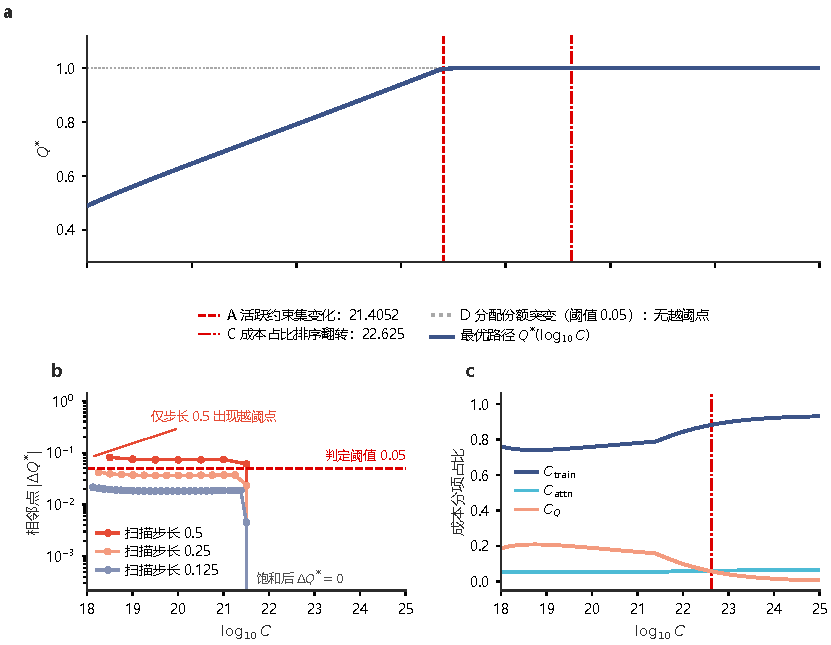
\includegraphics[width=0.92\linewidth]{figures/fig_q3_transition_definitions.pdf}
  \caption{结构性转移的三种定义及其识别结果。
  (a) 最优质量 $Q^{*}$ 随 $\log_{10}C$ 的路径；红色虚线为定义 A 的位置 21.4052，
  红色点划线为定义 C 的翻转位置 22.625，灰色虚线为定义 D 在 $\delta=0.05$ 下的阈值（细网格上无越阈点）。
  (b) 三种扫描步长下相邻点的 $|\Delta Q^{*}|$，横轴为 $\log_{10}C$，纵轴为对数刻度，
  阈值线为 0.05，仅步长 0.5 出现越阈点。
  (c) 三项成本占比随 $\log_{10}C$ 的演化，点划线标出 22.625 处 $C_{Q}$ 与 $C_{\text{attn}}$ 的排序翻转。}
  \label{fig:q3-transition}
\end{figure}

\subsection{成本函数与上下文长度的敏感性}
\label{subsec:q3-sensitivity}

题目要求讨论成本函数 $g$ 的选取对最优解的影响，三类 $g$ 在三个预算档下的最优质量列于表~\ref{tab:q3-costform}。

\begin{table}[htbp]
  \centering
  \caption{三类质量成本函数在各预算档下的最优质量（末行按列给出跨形式极差）}
  \label{tab:q3-costform}
  \begin{tabular}{@{}lccc@{}}
    \toprule
    成本函数 & $C=10^{19}$ & $C=10^{22}$ & $C=10^{24}$ \\
    \midrule
    指数型 $g=10^{7}\mathrm{e}^{6Q}$        & 0.6460 & 1.0000 & 1.0000 \\
    幂函数型 $g=5\times10^{9}Q^{4}$          & 0.5390 & 1.0000 & 1.0000 \\
    对数渐进型 $g=2\times10^{9}\ln(1+10Q)$   & 1.0000 & 1.0000 & 1.0000 \\
    \midrule
    跨形式极差                              & 0.4610 & 0.0 & 0.0 \\
    \bottomrule
  \end{tabular}
\end{table}

影响集中在预算紧张时。$C=10^{19}$ 档三类形式给出三种最优质量：指数型 $0.6460$、幂函数型 $0.5390$、对数渐进型 $1.0000$，跨形式极差为 $0.4610$；而 $C=10^{22}$ 与 $10^{24}$ 档下三者完全一致，均为 $1.0000$，分支同为上界分支。差额只出现在最低预算档，而该档恰是唯一存在内点最优的档位。

成因可由式~\eqref{eq:q3-R2} 读出：三类 $Q\,g'(Q)$ 的增长速度不同，幂函数型最快，指数型次之，对数渐进型以 $c$ 为上界；同一预算下三者的 $N^{*}$ 量级相近、右端相近，故增长越快的形式只能在越低的 $Q$ 处与右端相等。预算上升使右端抬高，三类形式被推向上界的过程彼此靠拢，至 $C\ge10^{22}$ 时给出相同读数。该比较在题给参数下成立，本节未重新标定三类形式，故不构成关于成本函数形式族的一般结论。质量成本函数的形式携带一层未经本数据检验的成分，这一处境与已有观察一致：固定算力下数据筛选比例本身服从标度关系，并非越高越好\citep{goyal2024filtering}，标度指数也并非先验常数\citep{bahri2024}。

题目「或改进 $g(Q)$」部分的分析结果如下。另取饱和指数型 $g=\gamma(1-\mathrm{e}^{-\lambda Q})$（$\gamma=10^{7}$，$\lambda=6.0$）、Hill 型 $g=\gamma Q^{\lambda}/(1+Q^{\lambda})$（同上参数）与二次型 $g=\gamma Q^{2}$（$\gamma=4.0343\times10^{9}$，$g(1)$ 与指数型相同）。两个有界型的边际成本在高 $Q$ 端趋于零，最优质量恒为上界 $1$，活跃约束集从不改变，按定义 A 判为无结构性转移；三条扫描各 57 个点的 KKT 判据全部通过，故不是求解失败。二次型给出双侧转移：低预算段 $Q^{*}$ 顶在下界 $Q_0$，中段为内点，高预算段顶在上界，成本分项占比排序在 $\log_{10}C=19.125$ 与 $22.5$ 各翻转一次；但定义 A 的识别法只检索 $Q\le1$ 一个谓词，二分定位不到左事件，且左事件本身是 $Q_0$ 这个人为下界的产物，而 $Q_0$ 尚未经外部确认。由这组对照可得有限结论：题给的三类 $g$ 不被上述两个方向的改进所取代——有界方向会使本问的核心发现消失，二次方向会引入依赖未确认参数的左侧事件；该表述限于这两个方向，不足以断言题给的三类 $g$ 是最优选择。

$L_{\text{ctx}}$ 经 $k=6+\eta L_{\text{ctx}}$ 进入成本。两类成本相等的临界尺度由 $C_{\text{attn}}/C_{\text{train}}=\eta L_{\text{ctx}}/6$ 定出，令其等于 1 得 $L_{\text{ctx}}^{\text{crit}}=6/\eta=30000$；该值只是两类开销相等的临界尺度，不是最优上下文长度，本节不把 $L_{\text{ctx}}$ 作为寻优变量。五档可行取值取自附件 C7，其中 $32768$ 与 $131072$ 位于临界之上，结果见图~\ref{fig:q3-lctx}，数值列于附录表~\ref{tab:app-q3-lctx}。

跨临界（$L_{\text{ctx}}$ 由 $2048$ 增至 $131072$）的后果可概括为显著压缩可负担规模、几乎不改变相对配比：$N^{*}$ 由 $5.6475$B 降至 $2.5507$B，降幅 $54.8351\%$；$D^{*}$ 由 $249.0624$B 降至 $116.1159$B，降幅 $53.3788\%$；$N^{*}{:}D^{*}$ 的相对极差仅 $3.22\%$，五档取值始终落在 $0.0220$ 至 $0.0227$ 的窄带内。原因见图~\ref{fig:q3-lctx}（c）：$C_{\text{attn}}/C_{\text{train}}$ 与三个决策变量均无关，只随 $L_{\text{ctx}}$ 由 $0.0683$ 线性升至 $4.3691$，预算中被注意力开销占去的部分显著增加，可支付的规模因此被压缩，而训练开销与质量开销之间的相对权衡未被重排。两项读数的性质不同，不宜互相替代：配比未重排不等于 $L_{\text{ctx}}$ 不重要。一种常见的近似是把 $L_{\text{ctx}}$ 视为对有效预算的整体缩放；该近似随 $L_{\text{ctx}}$ 增大而失效，本节不采用它解释上述读数，失效的解析原因仍在成本侧的不对称——$C_{Q}$ 只随 $D$ 缩放而不随 $ND$ 缩放。

\begin{figure}[htbp]
  \centering
  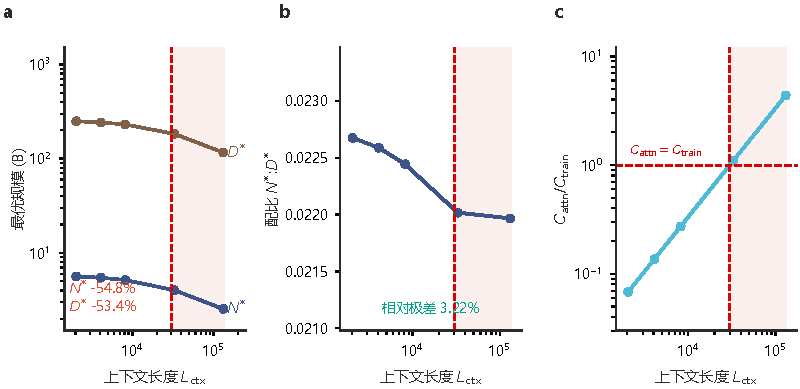
\includegraphics[width=0.96\linewidth]{figures/fig_q3_lctx_compression.pdf}
  \caption{上下文长度跨临界的影响，横轴为 $L_{\text{ctx}}$（token，对数刻度），红色虚线为临界值 30000，
  右侧阴影为位于临界之上的两档。
  (a) 最优规模 $N^{*}$ 与 $D^{*}$（B），纵轴为对数刻度，两档的降幅为 54.8351\% 与 53.3788\%；
  (b) 最优配比 $N^{*}{:}D^{*}$，纵轴为线性刻度，五档的相对极差为 3.22\%；
  (c) 注意力开销与训练开销之比 $C_{\text{attn}}/C_{\text{train}}$，纵轴为对数刻度，
  红色虚线为两者相等的条件 $L_{\text{ctx}}=6/\eta=30000$。}
  \label{fig:q3-lctx}
\end{figure}

\subsection{与基线的对照}
\label{subsec:q3-baseline}

本文主方法（式~\eqref{eq:q3-problem} 的分支枚举解）记为 M1o，基线记为 M0o，取 Chinchilla 经验配置：$D/N$ 固定为 20（\citet{hoffmann2022} 的 Approach 1/2 给出的约 20 tokens/param），质量固定在 $Q_0$ 即不投入质量提升，$N$ 与 $D$ 由预算约束确定。三档的损失与差距构成列于表~\ref{tab:q3-baseline}。

\begin{table}[htbp]
  \centering
  \caption{与基线的同口径对照及差距分解（报告差距为 $L(\text{M0o})-L(\text{M1o})$，
  仅质量通道差距以诊断配置 M0o$'$ 为参照，配比口径差距为前两者之差）}
  \label{tab:q3-baseline}
  \small
  \begin{tabular}{@{}lcccccc@{}}
    \toprule
    预算 & M1o 损失 & M0o 损失 & 报告差距 & 仅质量通道 & 配比口径 & 配比口径占比 \\
    \midrule
    $C=10^{19}$ & 3.1468 & 3.2538 & 0.1070 & 0.0727 & 0.0344 & 32.1032\% \\
    $C=10^{22}$ & 2.1511 & 2.2457 & 0.0947 & 0.0685 & 0.0262 & 27.6584\% \\
    $C=10^{24}$ & 1.9139 & 1.9702 & 0.0563 & 0.0371 & 0.0191 & 34.0083\% \\
    \bottomrule
  \end{tabular}
\end{table}

三档上主方法的损失均低于基线，报告差距为 $0.1070$、$0.0947$ 与 $0.0563$。该差距不能整体归因于质量通道：M0o 的 $D/N$ 被固定为 20，而本律在相同预算下、不投入质量时自身的最优比值随预算漂移，实测为 $79.5910$、$155.5005$ 与 $243.0207$（$\log$-$\log$ 斜率为 $0.0969558$），分别为 20 的约 4 倍、8 倍与 12 倍。为分开两部分，另算诊断配置 M0o$'$：质量同样固定为 $Q_0$，配比放开为本律自身的最优比值，其损失恰等于主方法在 $Q=Q_0$ 下界分支上的取值，即它就是本律的无质量投入退化解。以它为参照，报告差距分解为「仅质量通道」与「配比口径」两项，后者占报告差距的 $32.1032\%$、$27.6584\%$ 与 $34.0083\%$；三个数需同时报出，只报报告差距会把它整体读作质量投入的收益，只报仅质量通道一项则会隐去基线口径本身带来的差距。M0o 不使用本律的参数，是外部经验配置；M0o$'$ 是本律自身的退化分支，不具备外部性，故本文维持 M0o 为正式基线，M0o$'$ 只作诊断参照。

把约 20 tokens/param 当作硬判据并不成立。该比例出自 $\alpha\approx\beta\approx0.5$ 的参数化，此时 $D/N$ 与预算无关；本律的指数组合对应 $\alpha\ne\beta$，$D/N$ 随预算漂移，以常数 20 为判据会拒绝本律自身的真最优解。此外，本律 B1 侧的形状参数与 Chinchilla Approach 3 的常数按十亿单位折算后在数值上几乎同一（相对差 $9.4\times10^{-6}$ 至 $4.4\times10^{-4}$），两者是同源参数的不同标定，以 Chinchilla 的数值对照本律因此不构成独立的外部锚点。本节只把 20 列为参照比例，不用作判据；所引比例出自 \citet{hoffmann2022}，其常数在本文写作时未逐项核对原文。

\subsection{配比的边际方向}
\label{subsec:q3-direction}

配比已固定为 $\boldsymbol{z}_{\boldsymbol{p}}=\boldsymbol{0}$，但各领域的边际方向可以报出，用于回答「若不改变总算力、只调整领域之间的分配，应向何处倾斜」。配比项对 $\boldsymbol{p}$ 的偏导与系数 $b_i$ 成正比，故
\begin{equation}
  \frac{\partial L/\partial p_i}{\partial L/\partial p_j}=\frac{b_i}{b_j},
  \label{eq:q3-dldp}
\end{equation}
该比值与标度常数 $\kappa$ 无关，因为 $\kappa$ 只以整体因子同时进入分子与分母；本问据此只报符号与排序，不报绝对量级，也不报最优配比。参照点取 $C=10^{22}$ 档的解 $(N^{*},D^{*},Q^{*})=(5.6475,\,249.0624,\,1.0000)$，17 个领域按边际损失由大到小的排序列于附录表~\ref{tab:app-q3-dldp}：边际损失最大的是 \texttt{philpapers}，最小的是 \texttt{dm\_mathematics}，与 \S\ref{subsec:q3-model} 中角点解把 $0.9999999999999927$ 的份额给 \texttt{dm\_mathematics} 的方向一致。该排序与问题二的域比值表同源，二者都由问题一配比模型的系数导出，故不构成对问题二结论的独立佐证，只可作一次内部一致性检查。领域之间确实存在结构性差异，最优权重取决于领域的语言性质与目标任务的匹配程度，配比因而可在较小规模上回归预测\citep{liu2024regmix}，也可在训练过程中动态调整\citep{xie2023doremi}。

本节结论的适用条件有三。其一，形状参数取自问题二的 B1 侧，其中 $\gamma$ 由半合成网格 B7 反解、$\gamma\approx1$ 是条件性结论；问题二遗留的尺度对齐问题同样适用，最优质量绑定在 B7 的设计刻度上，不能直接代入问题一的经验质量。其二，$Q_0=0.35$ 未经裁定；在问题一实测的域级质量范围 $[0.223306,0.381496]$ 内扫动时，$Q^{*}$ 的极差为 $0.0117$、转移位置移动 $0.005981$（约 $0.006$ 个 $\log_{10}$ 单位），均远小于相应的判别尺度，故在实测范围内 $Q_0$ 不改变本节的结构结论，但其取值未经裁定的状态不变。其三，$C=10^{24}$ 档为外推，其读数不构成可靠预测。
